\chapter{\xlabel{pol2_image}POL-2 Image Display}
\label{sec:display}

\section{\xlabel{gaia}GAIA}

The \starlink\ package \gaia\ can be used to inspect the results of the data reduction.
To plot the output vector catalogue onto the final total intensity map
first open up the I map in gaia:

\begin{terminalv}
% gaia iext.sdf
\end{terminalv}


In the main Gaia window, select the drop-down menu option \texttt{Image Analysis /
Polarimetry toolbox…}. This should launch a new toolbox window entitled
GAIA: Polarimetry. From this window, use the drop-down menu option
\texttt{File / Open} to load the file mycat.FIT. This should then populate the lower part of the
window with the contents of this polarimetry catalogue file.
Each of the vectors in this file will be automatically overlaid on the main image window
(see figure \ref{fig:gaia-plot-vectors1}).

\begin{figure}[t!]
\begin{center}
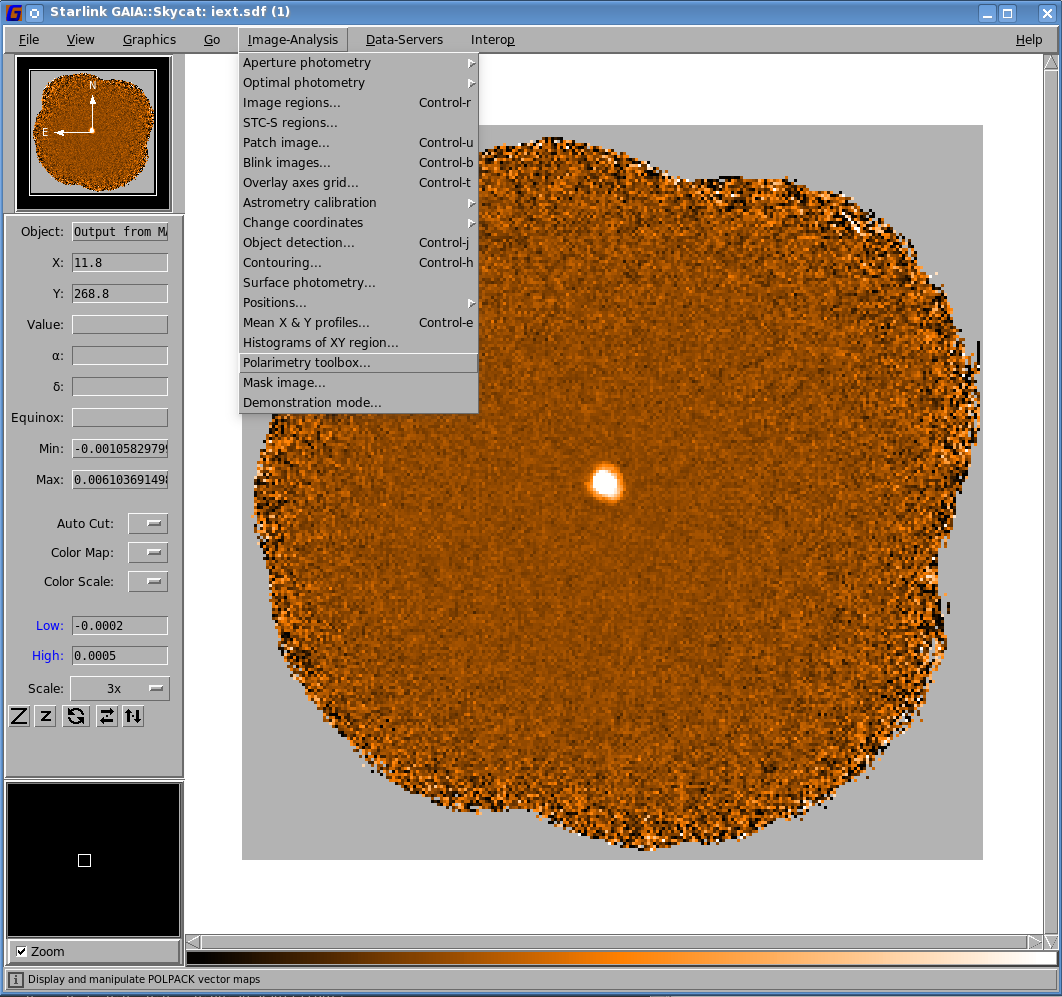
\includegraphics[width=0.46\linewidth]{sc22-gaia-plot-vectors-1.png}
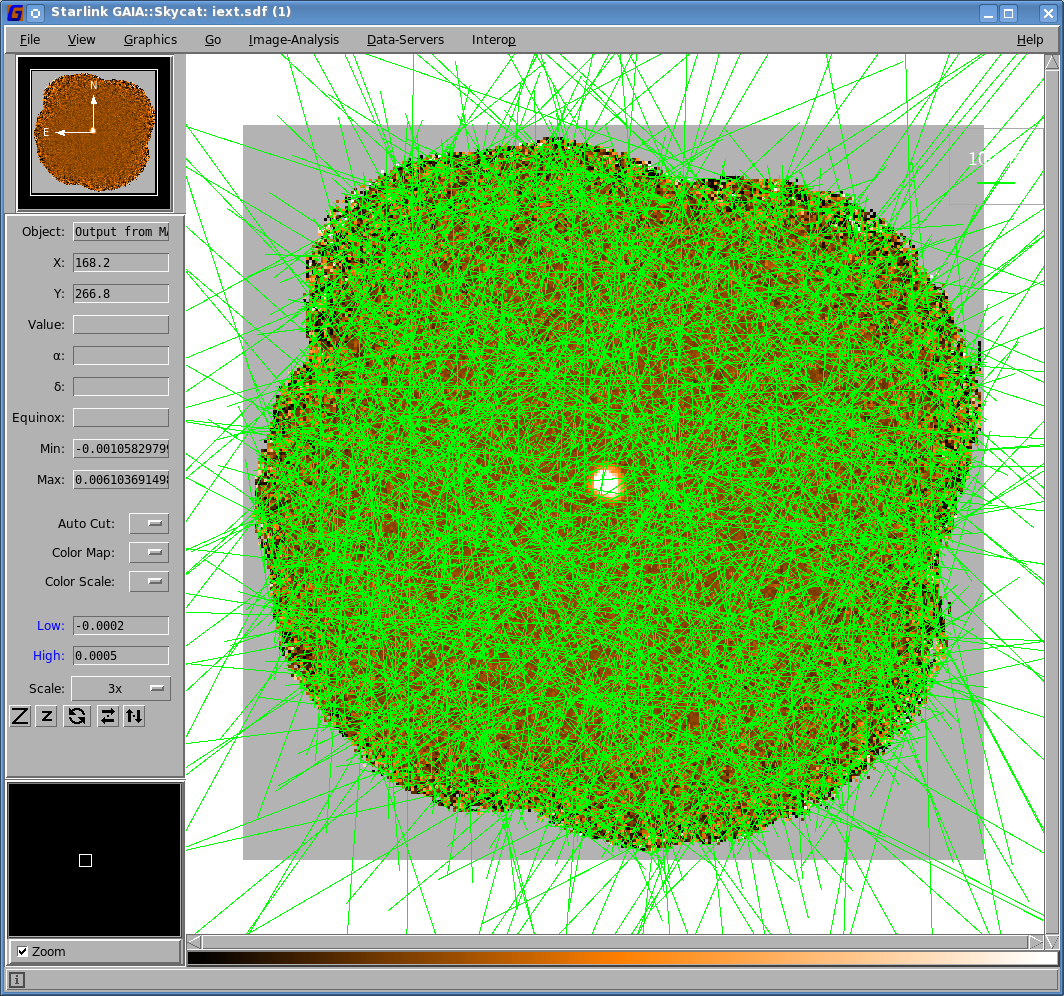
\includegraphics[width=0.46\linewidth]{sc22-gaia-plot-vectors-3.png}
\label{fig:gaia-plot-vectors1}
\caption [Over Plotting Vectors in GAIA]{
  \small Left: Opening up the polarimetry toolbox in GAIA. Right: The initial POL-2
vectors overplotted in GAIA.
}
\end{center}
\end{figure}

In order to filter the number of overlaid vectors down to a more useful number and size,
various options in the GAIA: Polarimetry window can be used. First, select the \texttt{Rendering}
tab on the left hand side. This will reveal a panel that will indicate which quantities
are currently being used for the vector overlays. In this case, the Vector length is taken
from the P column of the table, and the Vector angles are taken from the ANG column.

Currently the figure has too many vectors to be scientifically meaningful. To filter
out most of the extraneous vectors, click on the Selecting tab, and set the Expression
field to be the following:

\begin{terminalv}
$I/$DI<10
\end{terminalv}

\emph{Ensure you press return after entering in the above expression}.

The above expression selects the data points in the polarimetry table which have an
associated total intensity (column I) less than 10 times the
associated error value for that intensity (column DI). To remove all of these
extraneous vectors, either press control-X or use the drop-down menu option \texttt{Edit / Cut}.
This should leave just a small number of vectors clustering around the target object.

\begin{figure}[t!]
\begin{center}
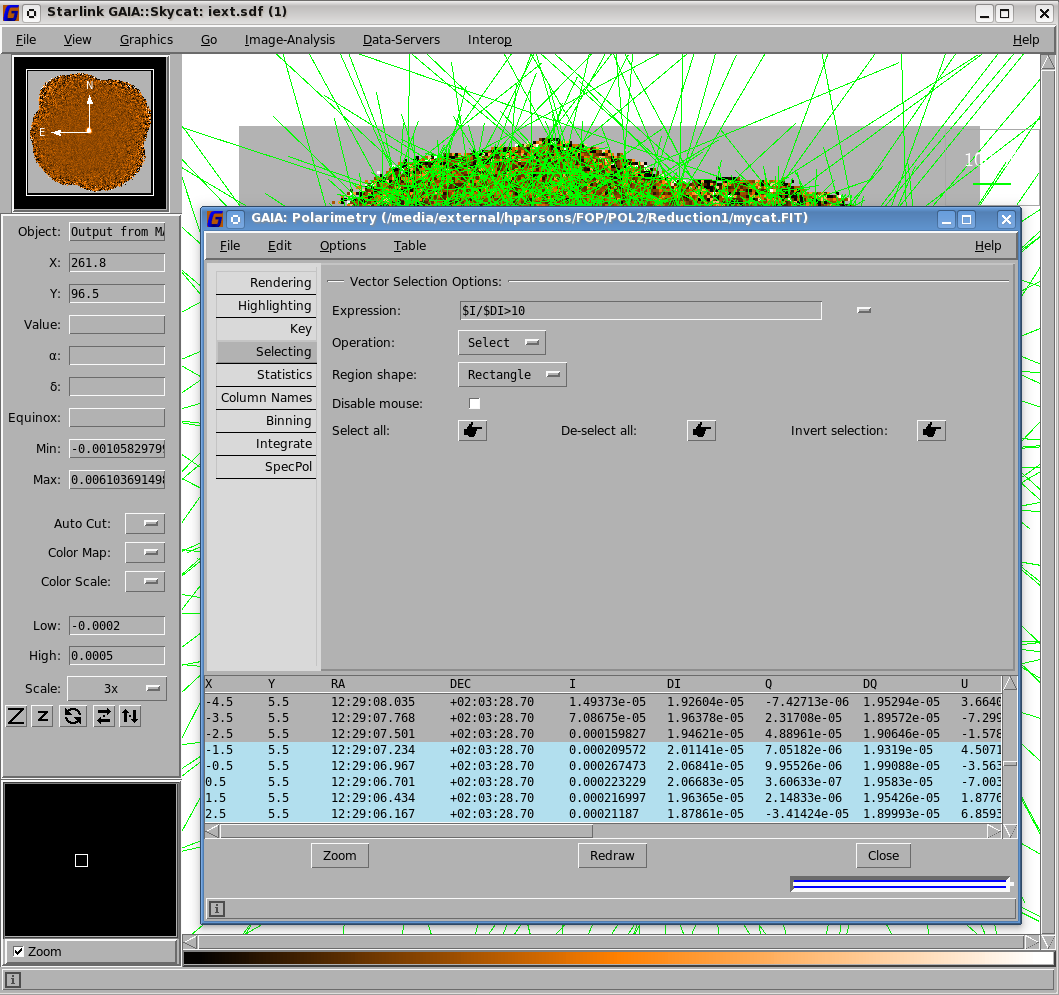
\includegraphics[width=0.46\linewidth]{sc22-gaia-plot-vectors-4.png}
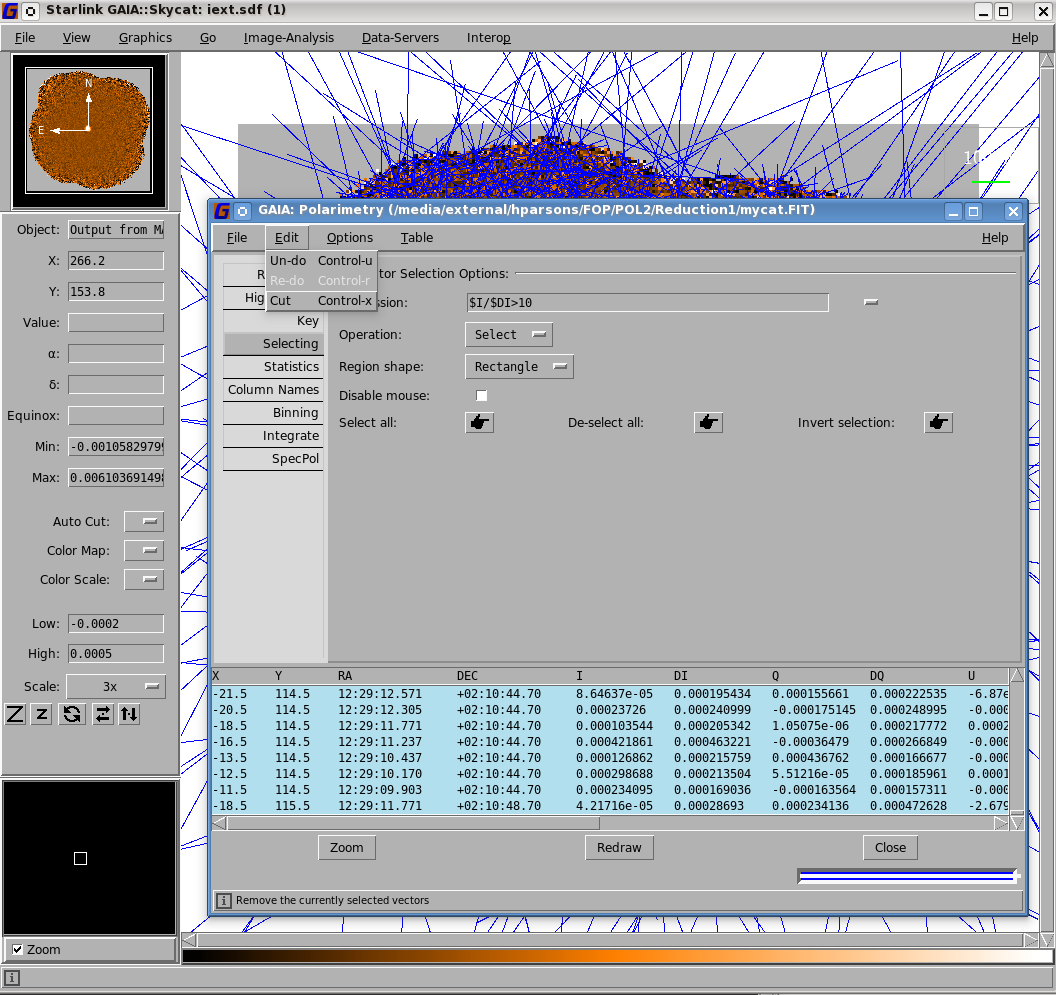
\includegraphics[width=0.46\linewidth]{sc22-gaia-plot-vectors-6.png}
\label{fig:gaia-plot-vectors2}
\caption [Selecting Vectors in GAIA]{
  \small Left: specifying vectors to display via the expression \$I/\$DI$>$10. This will only plot
vectors with an \SI{850}{\micro\metre} intensity signal-to-noise ratio grater than 10 in GAIA. To ensure thatthis is specified,
ensure you press the carriage return after entering the expression.
}
\end{center}
\end{figure}

Zooming in on the central region of the map, it can already be seen that the level of vector ordering
(and hence polarization) is quite low (see figure \ref{fig:gaia-plot-vectors3}). If needed it is
possible to change the scaling by selecting the Rendering tab in the GAIA: Polarimetry
window, and increasing the vector scale.


\begin{figure}[t!]
\begin{center}
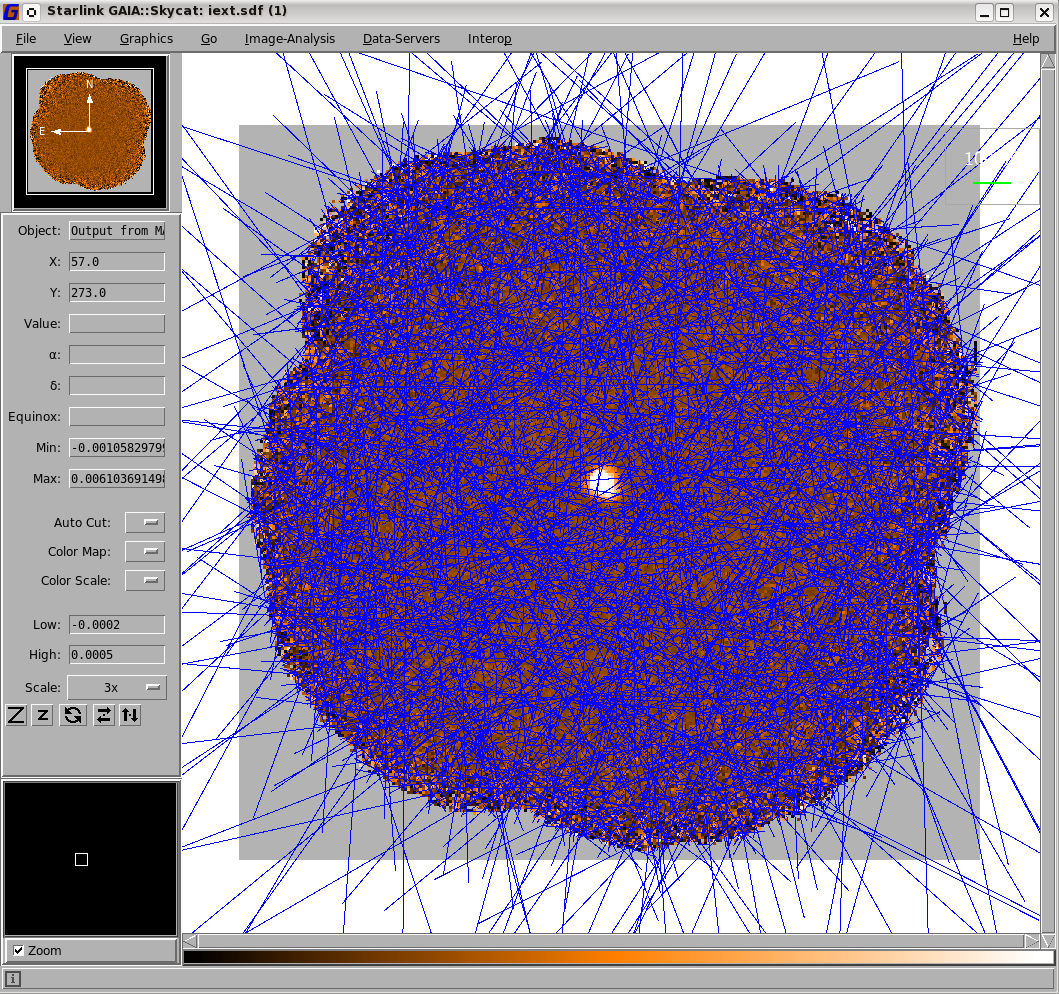
\includegraphics[width=0.44\linewidth]{sc22-gaia-plot-vectors-5.png}
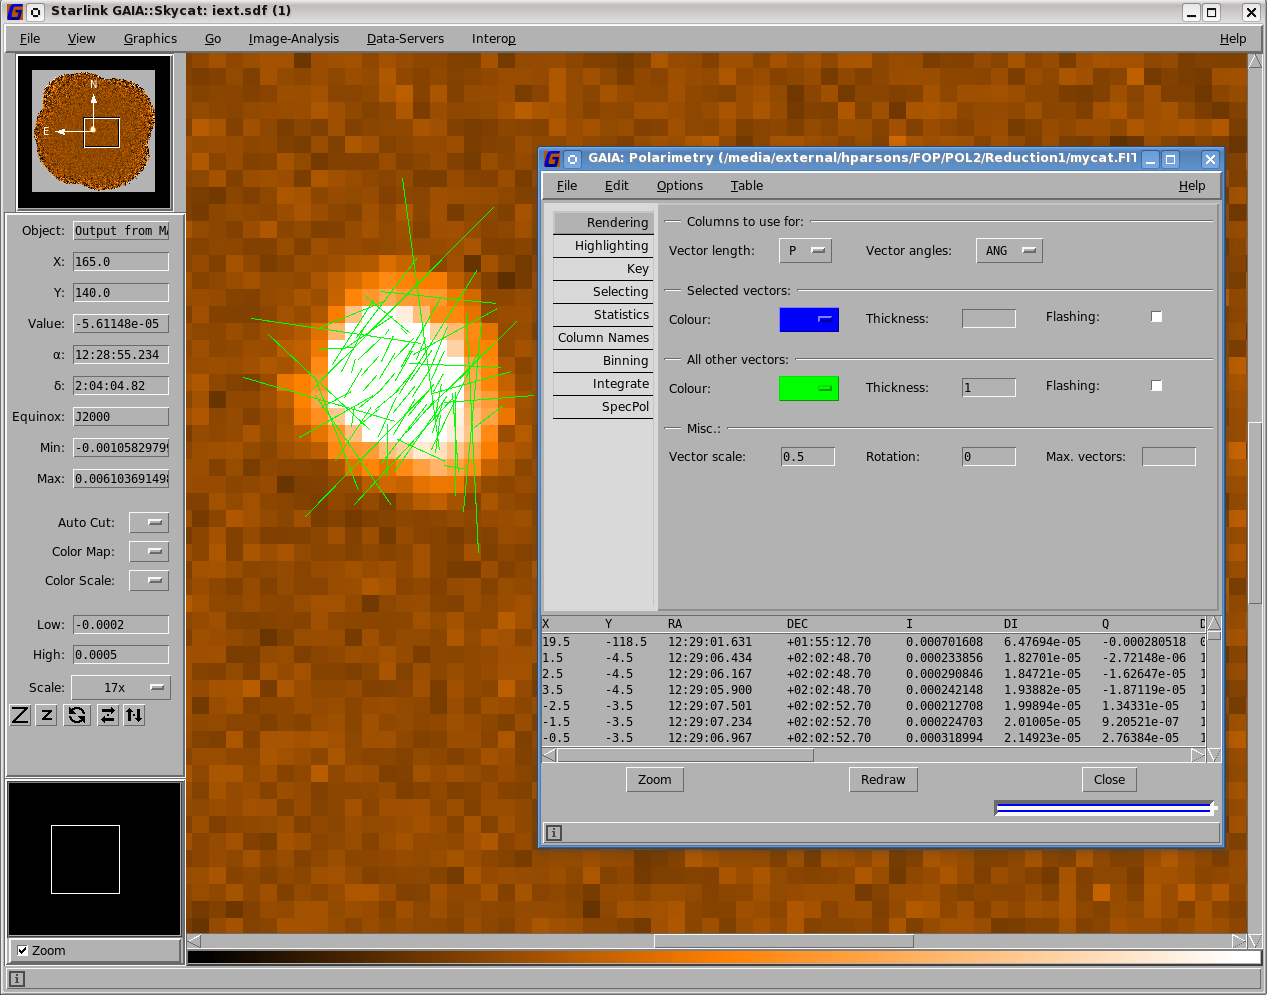
\includegraphics[width=0.52\linewidth]{sc22-gaia-plot-vectors-7.png}
\label{fig:gaia-plot-vectors3}
\caption [Over Plotting Vectors in GAIA]{
  \small Left: Selected vectors are marked in blue in this example, Right: after removal of selected
vectors all that remains are the vectors on the (zoomed) regions where \$I/\$DI$>$10.
}
\end{center}
\end{figure}


Finally it is useful for future use (as in the examples inthe following sections) to 
save the final selection of vectors. To save use the drop-down menue \texttt{File / Save} in 
the polarimetry toolbox.

\section{\xlabel{kappa}KAPPA and polpack}

It is possible to use \Kappa\ and polpack to create POL-2 plots.

\begin{terminalv}
% kappa
% polpack
\end{terminalv}

Note that in the following examples, it will be necessary to ensure that only the
vectors to be plotted are included in the file mycat.FIT.

There are two main ways to do this - either by saving the output catalogue
from GAIA or using the starlink package cursa to manipulate the catalogue you produced.
To use cursa simply run:

\begin{terminalv}
% cursa
\end{terminalv}

then to select the vectors of interest:

\begin{terminalv}
% catselect catin=mycat.FIT catout=selcat.FIT norejcat seltyp=e "expr='i>10*di'"
\end{terminalv}

it is also possible to crop images using catselect, by using the expression command. 
In this example we use only pixels above -10 on the y axis.

\begin{terminalv}
% catselect catin=mycat.FIT catout=selcat.FIT norejcat seltyp=e "expr='i>10*di and y>-10'"
\end{terminalv}




\begin{tip}
For a better font on pgplot postscript devices, set the
following environment variable. 

\begin{terminalv}
setenv PGPLOT_PS_FONT Times
\end{terminalv}

For more info, see

http://pipelinesandarchives.blogspot.com/2015/02/better-fonts-in-postscript-output-from.html

Graphics-related attributes that can be set are described at:

http://starlink.eao.hawaii.edu/docs/sun95.htx/sun95se28.html

and the coordinate system attributes that can be set are
described at:

http://starlink.eao.hawaii.edu/docs/sun95.htx/sun95se27.html
\end{tip}





\subsection{\xlabel{kappa-example1} Example 1 - a vector map with no background}
\label{section:kappa-example1}

In this section an output file: plot1.pdf is created from the input catalogue mycat.FIT

Select postscript graphics device, writing to file plot1.ps

\begin{terminalv}
gdset plot1.ps/acps
\end{terminalv}

For convenience, create a text file holding the main plotting style for polplot:

\begin{terminalv}
% cat sty
colour = black
drawtitle=0
format(1)=hms
format(2)=dms
\end{terminalv}

Likewise, create a text file holding the style for the vector length key:

\begin{terminalv}
% cat ksty
colour = black
drawtitle=0
\end{terminalv}


Plot the vector map (the \texttt{vscale} arameter controlls the vector
scale, and the \texttt{keyvec} parameter controls the length of the
vector used as the key. There are many other parameters that can be used
to control the behaviour of \texttt{polplot} - see the \polpack manual - SUN/223.

\begin{terminalv}
% polplot selcat.FIT  style=^sty keystyle=^ksty vscale=20 keyvec=20
\end{terminalv}

Convert the map into PDF file and remove blank margins (if required):

\begin{terminalv}
% ps2pdf plot1.ps temp.pdf
% pdfcrop temp.pdf plot1.pdf
\end{terminalv}


\begin{figure}[t!]
\begin{center}
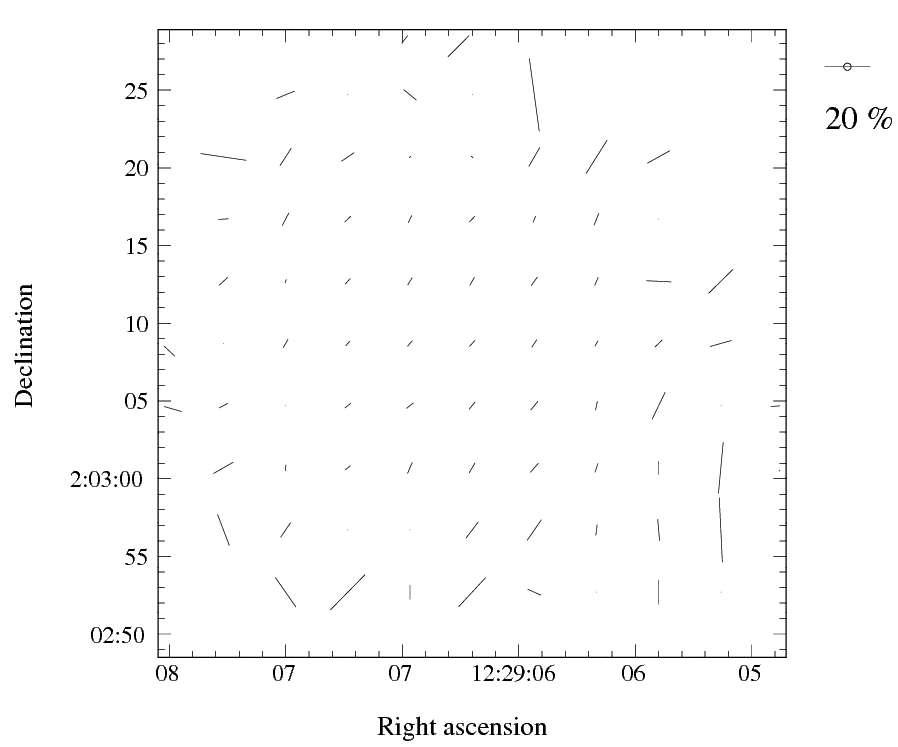
\includegraphics[width=0.75\linewidth]{sc22-kappa-plots-plot1.png}
\label{fig:kappa-plot1}
\caption [Vector map with polplot]{
  \small Result from Example 1: Producing a vector map with no background using polplot. 
}
\end{center}
\end{figure}

\subsection{\xlabel{kappa-example2} Example 2 - a vector map over a contour map}
\label{section:kappa-example2}


In this section we create an output file: plot2.pdf from the input catalogue mycat.FIT

\begin{terminalv}
% gdset plot2.ps/acps
\end{terminalv}

Setting up the main plotting style for contour and polplot:

\begin{terminalv}
% cat sty
colour = black
colour(curves)=red
width(curves)=3
drawtitle=0
format(1)=hms
format(2)=dms
\end{terminalv}


Produce the contour map

\begin{terminalv}
% contour iext\(0~150,0~200\) mode=perc percentiles=\[88,90,92,94,96,98\] style=^sty key=no
\end{terminalv}


Modify the above style for the vector map to produce black vectors

\begin{terminalv}
% cat vsty
^sty
colour(curves)=black
\end{terminalv}


Set the style for the vector length key:


\begin{terminalv}
% cat ksty
colour=black
width=3
drawtitle=0
\end{terminalv}

Plot the vector map over the contour map. The vectors and
contours are aligned automatically in sky coordinates:


\begin{terminalv}
% polplot selcat.FIT axes=no clear=no style=^vsty keystyle=^ksty vscale=20 keyvec=20
\end{terminalv}

Convert into a PDF file and remove blank margins (if required):

\begin{terminalv}
% ps2pdf plot2.ps temp.pdf
% pdfcrop temp.pdf plot2.pdf
\end{terminalv}

\begin{figure}[t!]
\begin{center}
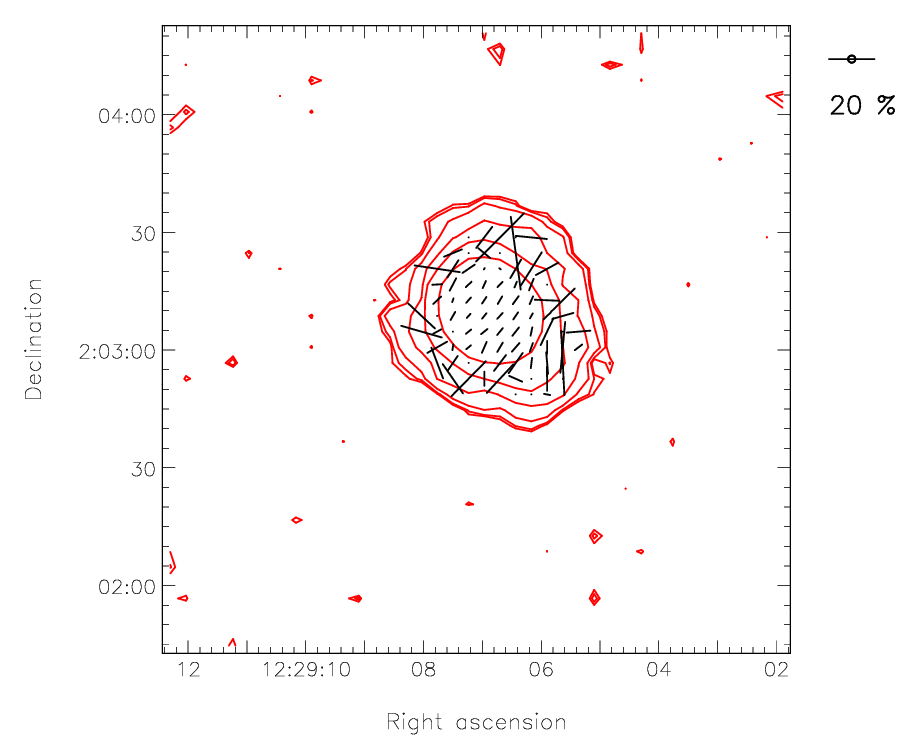
\includegraphics[width=0.75\linewidth]{sc22-kappa-plots-plot2.png}
\label{fig:kappa-plot2}
\caption [Vector map with contour map in polplot]{
  \small Result from Example 1: Producing a vector map over a contour map. 
}
\end{center}
\end{figure}

\subsection{\xlabel{kappa-example2} Example 3 - a vector map over a negative image}
\label{section:kappa-example3}


In this section we create an output file: plot3.pdf from the input catalogue mycat.FIT

\begin{terminalv}
% gdset plot3.ps/acps
\end{terminalv}


To ensure a monochrome colour table is used for the image:

\begin{terminalv}
% lutgrey
\end{terminalv}


Set the main plotting style for display and polplot:

\begin{terminalv}
% cat sty
colour = black
drawtitle=0
format(1)=hms
format(2)=dms
\end{terminalv}


The following function is used to reduce the dynamic range in the map (so
that we can see structure in the faint bits without saturating the
brightest regions).

\begin{terminalv}
maths "'((ia+0.0003)/0.14)**0.2'" ia=iext out=tmp1
\end{terminalv}


Display the negative image, using a reduced range of colours
(pens) so that the brightest regions are grey rather than black.
This means the black vectors can still be seen over the brightest
regions:

\begin{terminalv}
% display tmp1\(5~150,0~200\) mode=perc percentiles=\[2,98\] style=^sty \
        low=0.4 high=1.0
        penrange=\[0.4,1.0\]
\end{terminalv}


Modify the above style for the vector map to produce wider vectors:

\begin{terminalv}
% cat vsty
^sty
width(curves)=3
\end{terminalv}


Set the style for the vector length key:

\begin{terminalv}
% cat ksty
colour=black
width=3
drawtitle=0
\end{terminalv}


Plot the vector map over the contour map. The vectors are aligned automatically with the map.

\begin{terminalv}
% polplot selcat.FIT axes=no clear=no style=^vsty keystyle=^ksty vscale=20 keyvec=20
\end{terminalv}


Convert into a PDF file and remove blank margins (if required).

\begin{terminalv}
% ps2pdf plot3.ps temp.pdf
% pdfcrop temp.pdf plot3.pdf
\end{terminalv}


\begin{figure}[t!]
\begin{center}
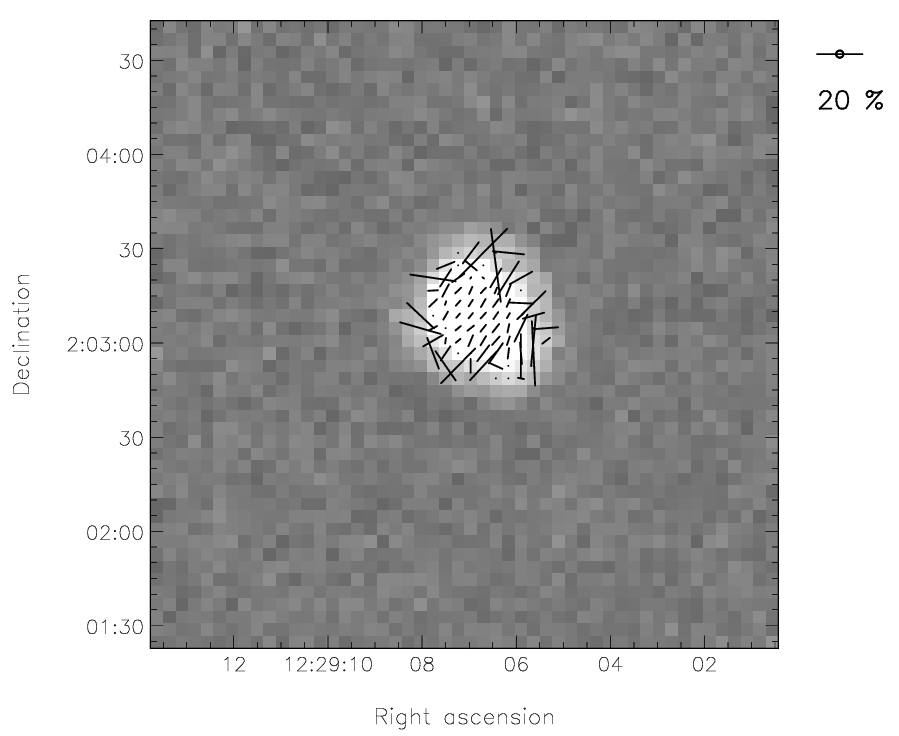
\includegraphics[width=0.75\linewidth]{sc22-kappa-plots-plot3.png}
\label{fig:kappa-plot3}
\caption [Vector map with negative image in polplot]{
  \small Result from Example 1: Producing a vector map over a negative image. 
}
\end{center}
\end{figure}


